%\documentclass[12pt,aspectratio=169]{beamer}
\documentclass[12pt]{beamer}

\usetheme{metropolis}
\setbeamertemplate{bibliography item}{\insertbiblabel}
\usepackage{xcolor}
\usepackage{appendixnumberbeamer}
\usepackage{verbatim}
\usepackage{caption}
\usepackage{minted}
\setsansfont[BoldFont={Fira Sans Bold}, ItalicFont={Fira Sans Italic}]{Fira Sans Regular}
\usepackage[backend=biber,style=ieee]{biblatex}
\usepackage{hyperref}
%\bibliography{references}
\graphicspath{{./figs/}}
\setlength{\belowcaptionskip}{-10pt}
\setbeamersize{text margin left=5mm,text margin right=7mm}

\title{EECS 151/251A: Discussion 1}
\subtitle{Intro, Boolean Algebra, Verilog Basics}
\author{}
\date{8/30/2019}

\begin{document}
\begin{frame}
    \maketitle
\end{frame}

\begin{frame}{Intro}
  \begin{itemize}
  \setlength\itemsep{0.75em}
    \item A bit about me
    \item Each discussion will review the week's lectures and provide a few examples and questions to solve
    \item All labs, discussions, and lectures will be posted on the website \url{http://inst.eecs.berkeley.edu/~eecs151/fa19/}
    \item All instructor and TA office hours are on the website
    \item Sign up for Piazza \url{https://piazza.com/class/jzjemj1hg0z2nj}
    \item No textbook required. Digital Integrated Circuits (Rabaey) is helpful.
  \end{itemize}
\end{frame}

\begin{frame}{Pre-Reqs}
  \begin{itemize}
  \setlength\itemsep{0.75em}
    \item CS61C
      \begin{itemize}
        \item C
        \item digital logic
        \item RISC-V ISA
        \item 3/5-stage CPU pipeline
        \item hazard handling
      \end{itemize}
    \item EE16A/B
      \begin{itemize}
        \item RC circuits
        \item energy and power
      \end{itemize}
  \end{itemize}
\end{frame}

\begin{frame}{Scaling}
  \begin{itemize}
    \item \textit{Moore's Law}: Number of transistors per chip doubles every two years $\rightarrow$ cost per transistor is halved.
      \begin{itemize}
        \item Cost isn't going down anymore when scaling to a new node
        \item But increasing die size and chiplet packaging can keep the trend alive
      \end{itemize}
      \vspace{0.5cm}
    \begin{columns}
    \begin{column}{0.5\textwidth}
        \begin{center}
         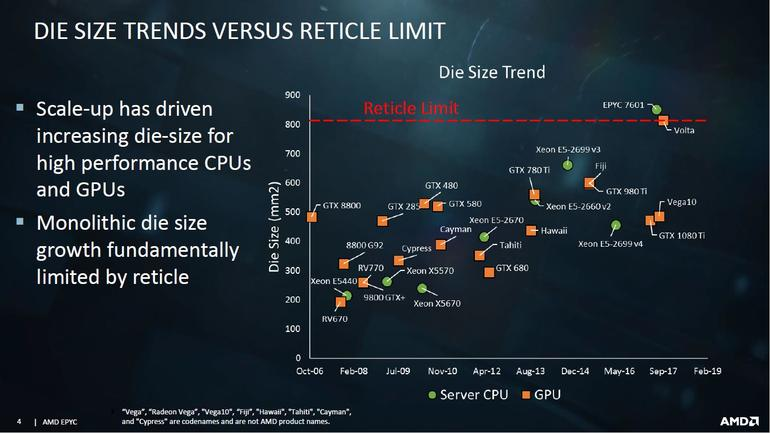
\includegraphics[width=\textwidth]{amd_die_size.jpg}
         \end{center}
    \end{column}
    \begin{column}{0.5\textwidth}  %%<--- here
        \begin{center}
         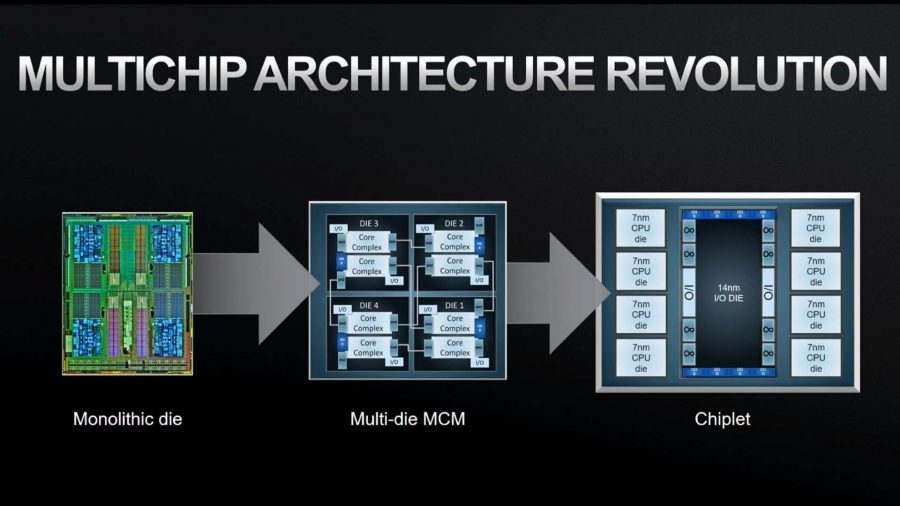
\includegraphics[width=\textwidth]{amd_mcm.jpg}
         \end{center}
    \end{column}
    \end{columns}
  \end{itemize}
\end{frame}

\begin{frame}{Wafer-Scale Integration}
  \begin{itemize}
    \item Startup Cerebras presented a wafer-scale ML accelerator at HotChips this year
    \item Defects always exist on such a large scale, need redundancy
    \item Consumes \textbf{15 kW}! Custom cooling solution and power delivery required
  \end{itemize}
  \begin{center}
   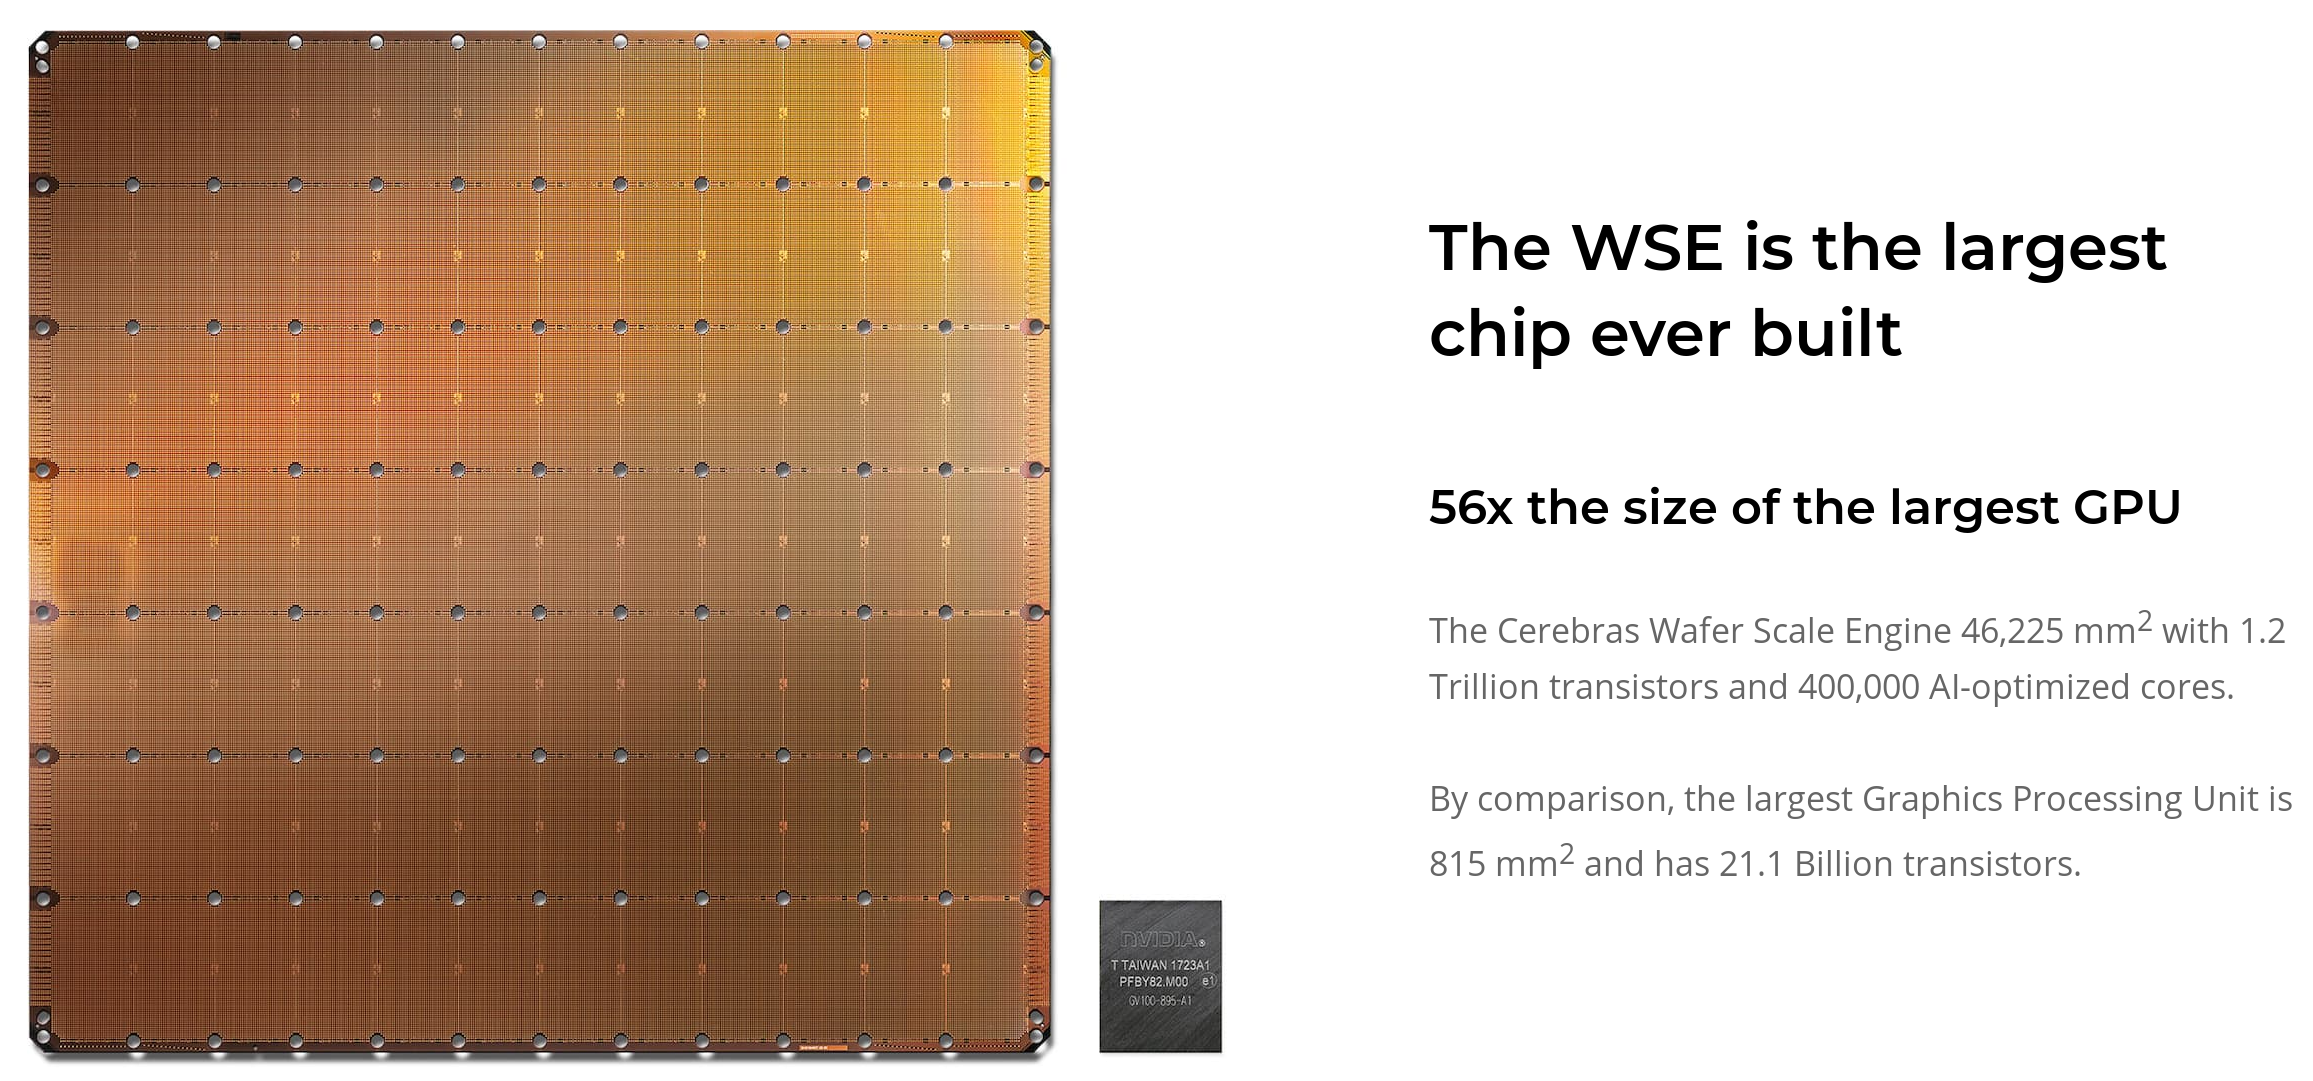
\includegraphics[width=0.7\textwidth]{cerebras.png}
  \end{center}
\end{frame}

\begin{frame}{Scaling}
  \begin{itemize}
    \item \textit{Dennard Scaling}: As MOSFETs scale down, voltages and currents scale proportionally and power density stays constant
      \begin{itemize}
        \item Delay $\approx C \cdot V / I_{avg}$ (scales down linearly with transistor shrink)
        \item $P \approx C \cdot V^2 / \text{Delay}$ (scales down quadratically)
      \end{itemize}
      \vspace{0.5cm}
      \begin{figure}
        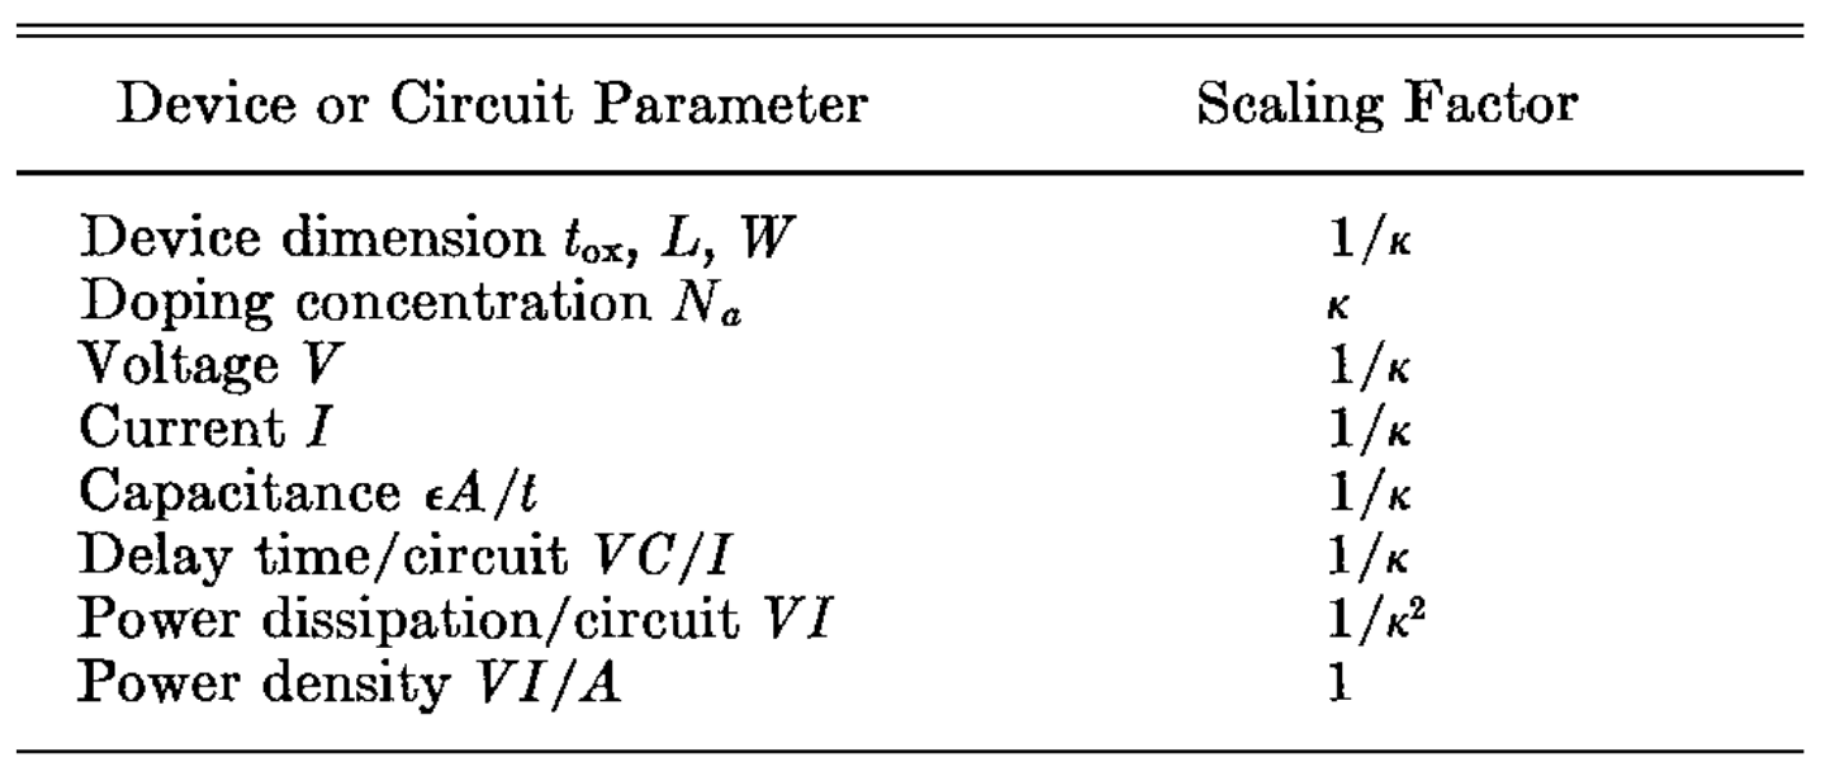
\includegraphics[width=0.6\textwidth]{dennard.png}
      \end{figure}
  \end{itemize}
\end{frame}

%\begin{frame}{Failure of Dennard Scaling}
%\end{frame}

\begin{frame}{Logic Operators}
  \begin{itemize}
    \item Logic operators work over boolean symbols
    \item Common boolean operators include AND, OR, and NOT
    \item We will usually write AND as `multiplication', OR as `addition', and NOT with an overline
    \item e.g. A AND B OR (NOT C) $= AB + \overline{C}$
    \item Logic operators in boolean expressions map to digital logic gates (a key abstraction)
  \end{itemize}
\end{frame}

\begin{frame}{Boolean Algebra}
  \begin{itemize}
    \item Review some basic boolean algebra laws
    \item OR Identity: $A + 1 = 1$, $A + 0 = A$, $A + \overline{A} = 1$
    \item AND Identity: $A1 = A$, $A0 = 0$, $A\overline{A} = 0$
    \item Absorption: $A + AB = A$, $A(A + B) = A$
    \item DeMorgan's Laws: $\overline{A + B} = \overline{A}\; \overline{B}$, $\overline{AB} = \overline{A} + \overline{B}$
  \end{itemize}
\end{frame}

\begin{frame}{Verilog}
  \begin{itemize}
    \item Check out the \href{http://inst.eecs.berkeley.edu/~eecs151/fa19/files/verilog/Verilog_Primer_Slides.pdf}{Verilog Primer Slides} before Lab 2
  \end{itemize}
\end{frame}

\end{document}
